\begin{figure}[htbp]
\centering
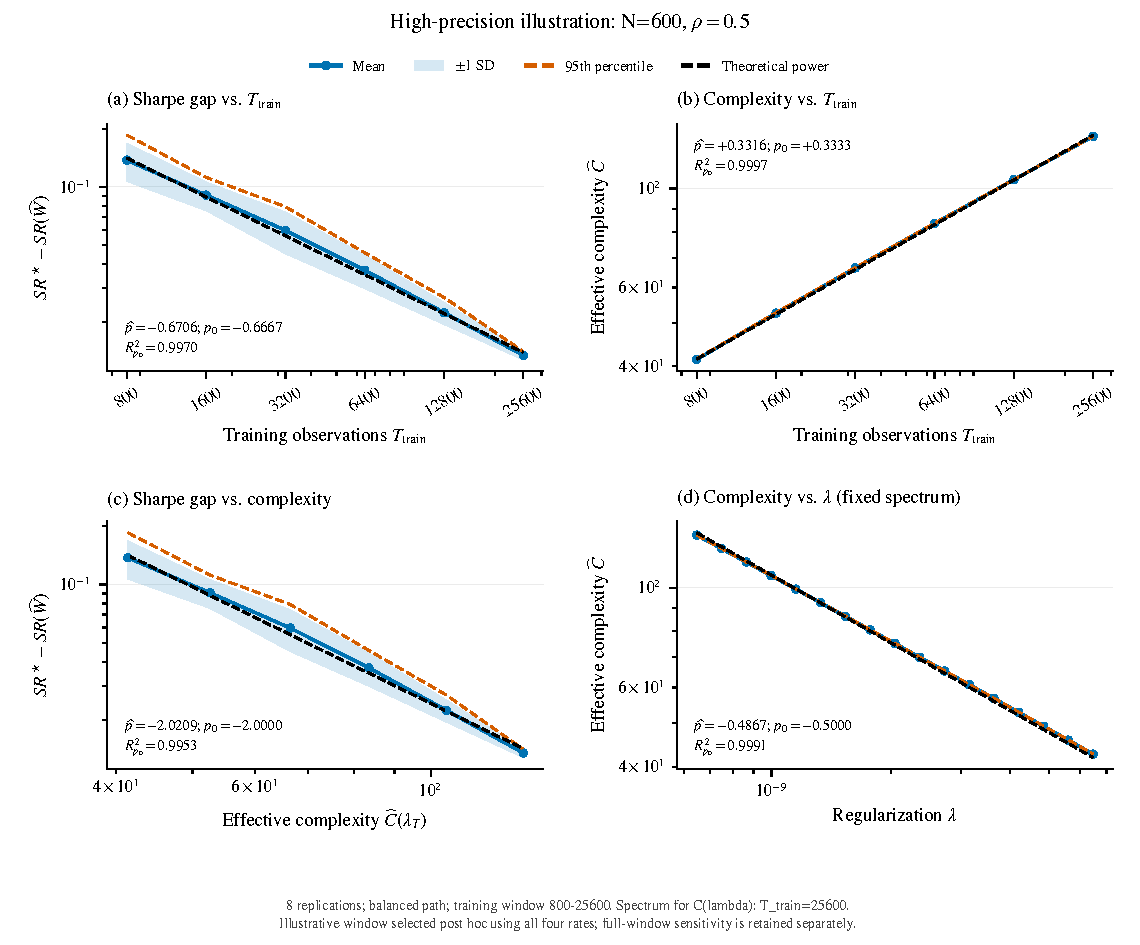
\includegraphics[width=\linewidth]{../simulations/outputs/paper_selection_v1/high_precision_rates.pdf}
\caption{Higher-precision illustration. $N=600$, $\rho=0.5$, Nystr\"om rank 8192,
8 replications, and $T_{\mathrm{train}}\in[800,25600]$.
The regularization follows the balanced path $\lambda_T=C_0T_{\mathrm{train}}^{-2/3}$.
The scale is $C_0=5.623413\times10^{-7}$.
Means, one sample standard deviation across replications, and empirical 95th percentiles of the displayed ordinates are shown.
The black curves fit one amplitude with the theoretical exponent fixed and no intercept;
$\widehat p$ is the unrestricted log--log slope of the mean curve.
In panel (c), horizontal bars are one SD of complexity; percentile ordinates are placed at mean complexity.
For $C(\lambda)$, the training spectrum is held fixed at $T_{\mathrm{train}}=25600$.
This illustrative specification was selected after observing the simulations: one common cutoff
minimizes the largest relative discrepancy of the four exponents, subject to all fixed-power
$R^2\geq0.99$. The rank of the higher-precision study was fixed separately by its complexity-error
certificate. This is a descriptive comparison; the primary cutoff of 1600 and all sensitivity
results remain available in the full simulation reports.}
\label{fig:simulation-high-precision}
\end{figure}

\begin{figure}[htbp]
\centering
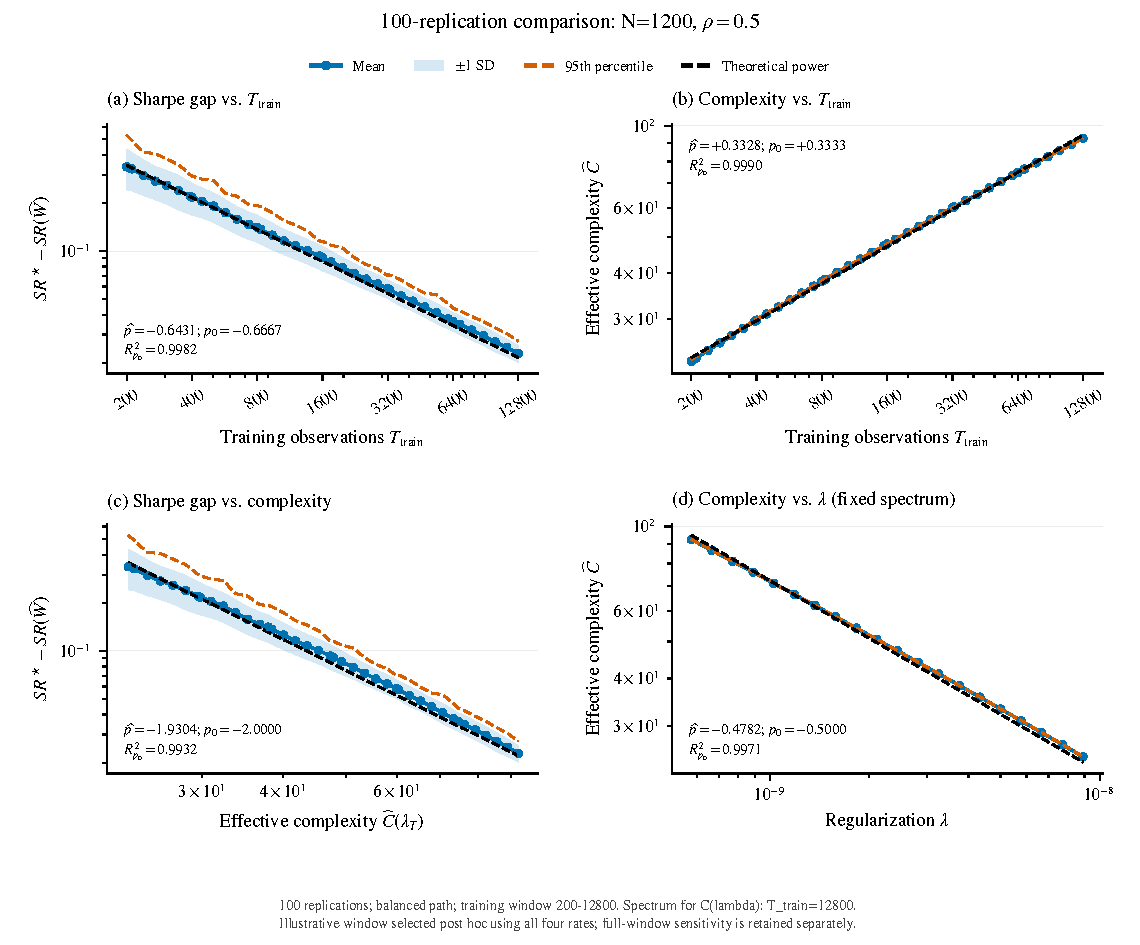
\includegraphics[width=\linewidth]{../simulations/outputs/paper_selection_v1/confirmation_rates.pdf}
\caption{Comparison with 100 Monte Carlo replications. $N=1200$, $\rho=0.5$, Nystr\"om rank 1024,
100 replications, and $T_{\mathrm{train}}\in[200,12800]$.
The regularization follows the balanced path $\lambda_T=C_0T_{\mathrm{train}}^{-2/3}$.
The scale is $C_0=3.162278\times10^{-7}$.
Means, one sample standard deviation across replications, and empirical 95th percentiles of the displayed ordinates are shown.
The black curves fit one amplitude with the theoretical exponent fixed and no intercept;
$\widehat p$ is the unrestricted log--log slope of the mean curve.
In panel (c), horizontal bars are one SD of complexity; percentile ordinates are placed at mean complexity.
For $C(\lambda)$, the training spectrum is held fixed at $T_{\mathrm{train}}=12800$.
This illustrative specification was selected after observing the simulations: one common cutoff
minimizes the largest relative discrepancy of the four exponents, subject to all fixed-power
$R^2\geq0.99$. The rank of the higher-precision study was fixed separately by its complexity-error
certificate. This is a descriptive comparison; the primary cutoff of 1600 and all sensitivity
results remain available in the full simulation reports.}
\label{fig:simulation-confirmation}
\end{figure}
